

%%%%%%%%%%%%%%%%%%%%%%%%%%%%%%%%%%%%%%%%%%%%%%%%%%%%%%%%%%%%

%&latex
\documentclass[12pt]{article}
\usepackage[USenglish]{babel}
\usepackage{graphicx}
\usepackage{setspace}
\usepackage{varioref}
\usepackage{booktabs}
\usepackage{xfrac}
\usepackage{longtable} % use for tables going over more than one page

\usepackage[osf,sc]{mathpazo} % Use the Palatino font
%\usepackage[T1]{fontenc} % Use 8-bit encoding that has 256 glyphs
%\linespread{1.05} % Line spacing - Palatino needs more space between lines
\linespread{1.2} % Line spacing - Palatino needs more space between lines
\usepackage{microtype} % Slightly tweak font spacing for aesthetics
\usepackage[hmarginratio=1:1,top=32mm,left=1cm, right=1cm, columnsep=10pt]{geometry} % Document margins
%\usepackage{multicol} % Used for the two-column layout of the document
\usepackage[hang, small,labelfont=bf,up,textfont=it,up]{caption} % Custom captions under/above floats in tables or figures
\usepackage{booktabs} % Horizontal rules in tables
\usepackage{float} % Required for tables and figures in the multi-column environment - they need to be placed in specific locations with the [H] (e.g. \begin{table}[H])
\usepackage{hyperref} % For hyperlinks in the PDF
\usepackage{lettrine} % The lettrine is the first enlarged letter at the beginning of the text
\usepackage{paralist} % Used for the compactitem environment which makes bullet points with less space between them

\usepackage{amsfonts}
\usepackage{amsmath}
\usepackage{sub caption} %allows combination of figures
\usepackage{abstract} % Allows abstract customization
\renewcommand{\abstractnamefont}{\normalfont\bfseries} % Set the "Abstract" text to bold
%\renewcommand{\abstracttextfont}{\normalfont\small\itshape} % Set the abstract itself to small italic text

\usepackage{titlesec} % Allows customization of titles
%\renewcommand\thesection{\Roman{section}} % Roman numerals for the sections
%\renewcommand\thesubsection{\Roman{subsection}} % Roman numerals for subsections
\titleformat{\section}[block]{\large\scshape\centering}{\thesection.}{1em}{} % Change the look of the section titles
\titleformat{\subsection}[block]{\large}{\thesubsection.}{1em}{} % Change the look of the section titles
\usepackage{fancyhdr} % Headers and footers
%\pagestyle{fancy} % All pages have headers and footers
%\fancyhead{} % Blank out the default header
%\fancyfoot{} % Blank out the default footer
%\fancyfoot[RO,LE]{\thepage} % Custom footer text



\makeatletter
\def\input@path{{../tables/}}
\makeatother

\graphicspath{{../figures/}}

\usepackage{caption}

\captionsetup[table]{labelformat=empty}
\captionsetup[figure]{labelformat=empty}

%%%%%%%%%%%%%%%%%%%%%%%%%%%%%%%%%%%%%%%%%%%%%%%%%%%%%%%%%%%%


\begin{document}

\begin{table}[htbp]\centering
\def\sym#1{\ifmmode^{#1}\else\(^{#1}\)\fi}
\caption{Table 1. OLS}
\begin{tabular}{lcccccc}
    \input{table1.tex}
\end{tabular}
\end{table}


\begin{table}[htbp]\centering
\def\sym#1{\ifmmode^{#1}\else\(^{#1}\)\fi}
\caption{Table 2. OLS by bin}
\begin{tabular}{lcccccc}
    \input{table2.tex}
\end{tabular}
\end{table}

\begin{table}[htbp]\centering
\def\sym#1{\ifmmode^{#1}\else\(^{#1}\)\fi}
\caption{Table 3. IV binary v cts}
\begin{tabular}{lcccccc}
    \input{table3.tex}
\end{tabular}
\end{table}

\begin{table}[htbp]\centering
\def\sym#1{\ifmmode^{#1}\else\(^{#1}\)\fi}
\caption{Table 4. IV by bin, binary}
\begin{tabular}{lcccccc}
    \input{table4.tex}
\end{tabular}
\end{table}

\begin{table}[htbp]\centering
\def\sym#1{\ifmmode^{#1}\else\(^{#1}\)\fi}
\caption{Table 5. Balance check}
\begin{tabular}{lcc}
    \input{table5.tex}
\end{tabular}
\end{table}

\begin{table}[htbp]\centering
\def\sym#1{\ifmmode^{#1}\else\(^{#1}\)\fi}
\caption{Table 6. Residual Test}
\begin{tabular}{lccc}
  \input{table6.tex}
\end{tabular}
\end{table}



\begin{table}[htbp]\centering
\def\sym#1{\ifmmode^{#1}\else\(^{#1}\)\fi}
\caption{Table 7. Fiscal treatment regression, pooled probit estimators}
\begin{tabular}{lcccc}
    \input{table7.tex}
\end{tabular}
\end{table}

\begin{table}[htbp]\centering
\def\sym#1{\ifmmode^{#1}\else\(^{#1}\)\fi}
\caption{Table 8. AIPW full sample}
\begin{tabular}{lcccccc}
    \input{table8.tex}
\end{tabular}
\end{table}

\begin{table}[htbp]\centering
\def\sym#1{\ifmmode^{#1}\else\(^{#1}\)\fi}
\caption{Table 9. AIPW boom vs. slumps}
\begin{tabular}{lcccccc}
    \input{table9.tex}
\end{tabular}
\end{table}

\begin{table}[htbp]\centering
\def\sym#1{\ifmmode^{#1}\else\(^{#1}\)\fi}
\caption{Table A1. OLS with Country-Fixed Effects and Controlling for World Growth}
\begin{tabular}{lcccccc}
    \input{tableA1.tex}
\end{tabular}
\end{table}

\begin{table}[htbp]\centering
\def\sym#1{\ifmmode^{#1}\else\(^{#1}\)\fi}
\caption{Table A2. IV with Country-Fixed Effects and Controlling for World Growth, bin IV}
\begin{tabular}{lcccccc}
    \input{tableA2.tex}
\end{tabular}
\end{table}

\begin{table}[htbp]\centering
\def\sym#1{\ifmmode^{#1}\else\(^{#1}\)\fi}
\caption{Table A3. ATE robustness}
\begin{tabular}{lccccc}
    \input{tableA3.tex}
\end{tabular}
\end{table}

\begin{table}[htbp]\centering
\def\sym#1{\ifmmode^{#1}\else\(^{#1}\)\fi}
\caption{Table A4. Treatment on treatment}
\begin{tabular}{lccc}
    \input{tableA4.tex}
\end{tabular}
\end{table}

\newpage

\begin{figure}[h]\centering
\caption{Figure 1. IPWRA example}
    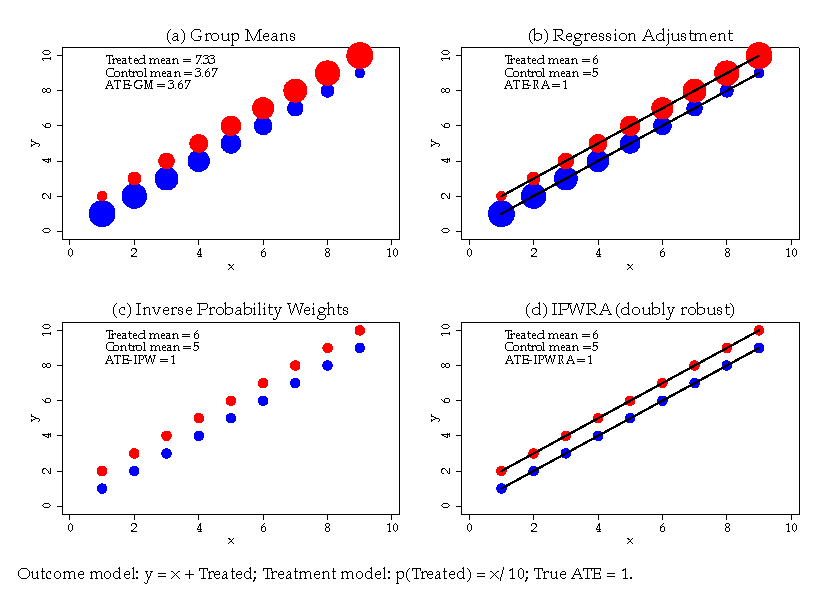
\includegraphics{figure1.pdf}
\end{figure}

\begin{figure}[h]\centering
\caption{Figure 2. Overlap}
    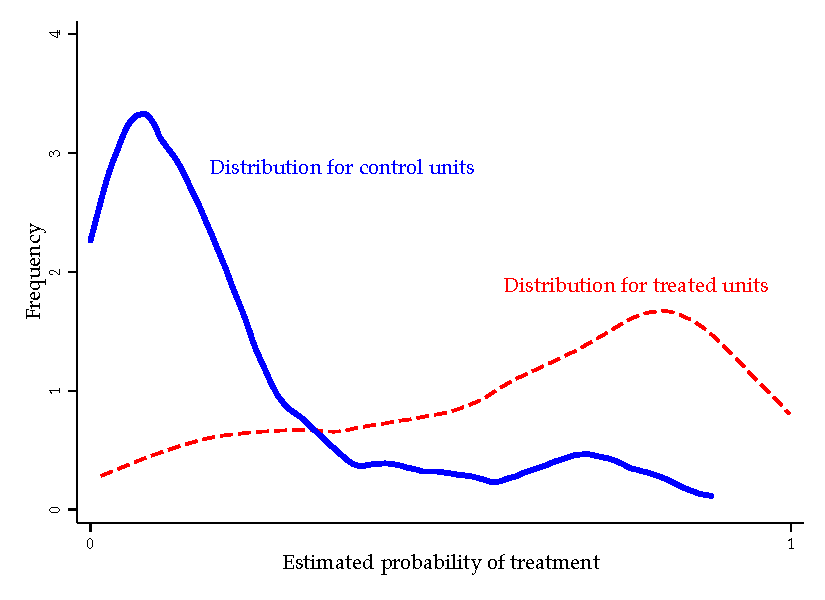
\includegraphics{figure2.pdf}
\end{figure}

\begin{figure}[h]\centering
\caption{Figure 3. LPs with unrestricted slopes}
    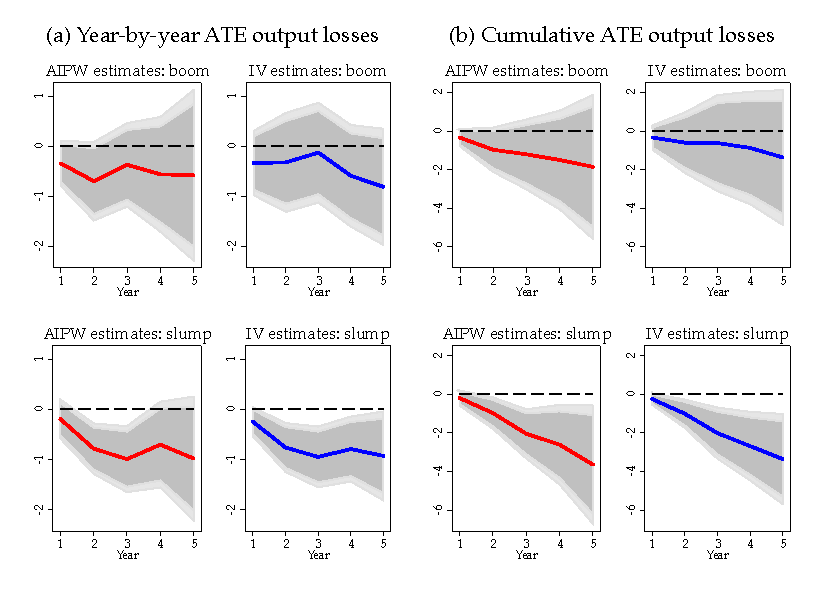
\includegraphics{figure3.pdf}
\end{figure}

\begin{figure}[h]\centering
\caption{Figure 4. UK counterfactual}
    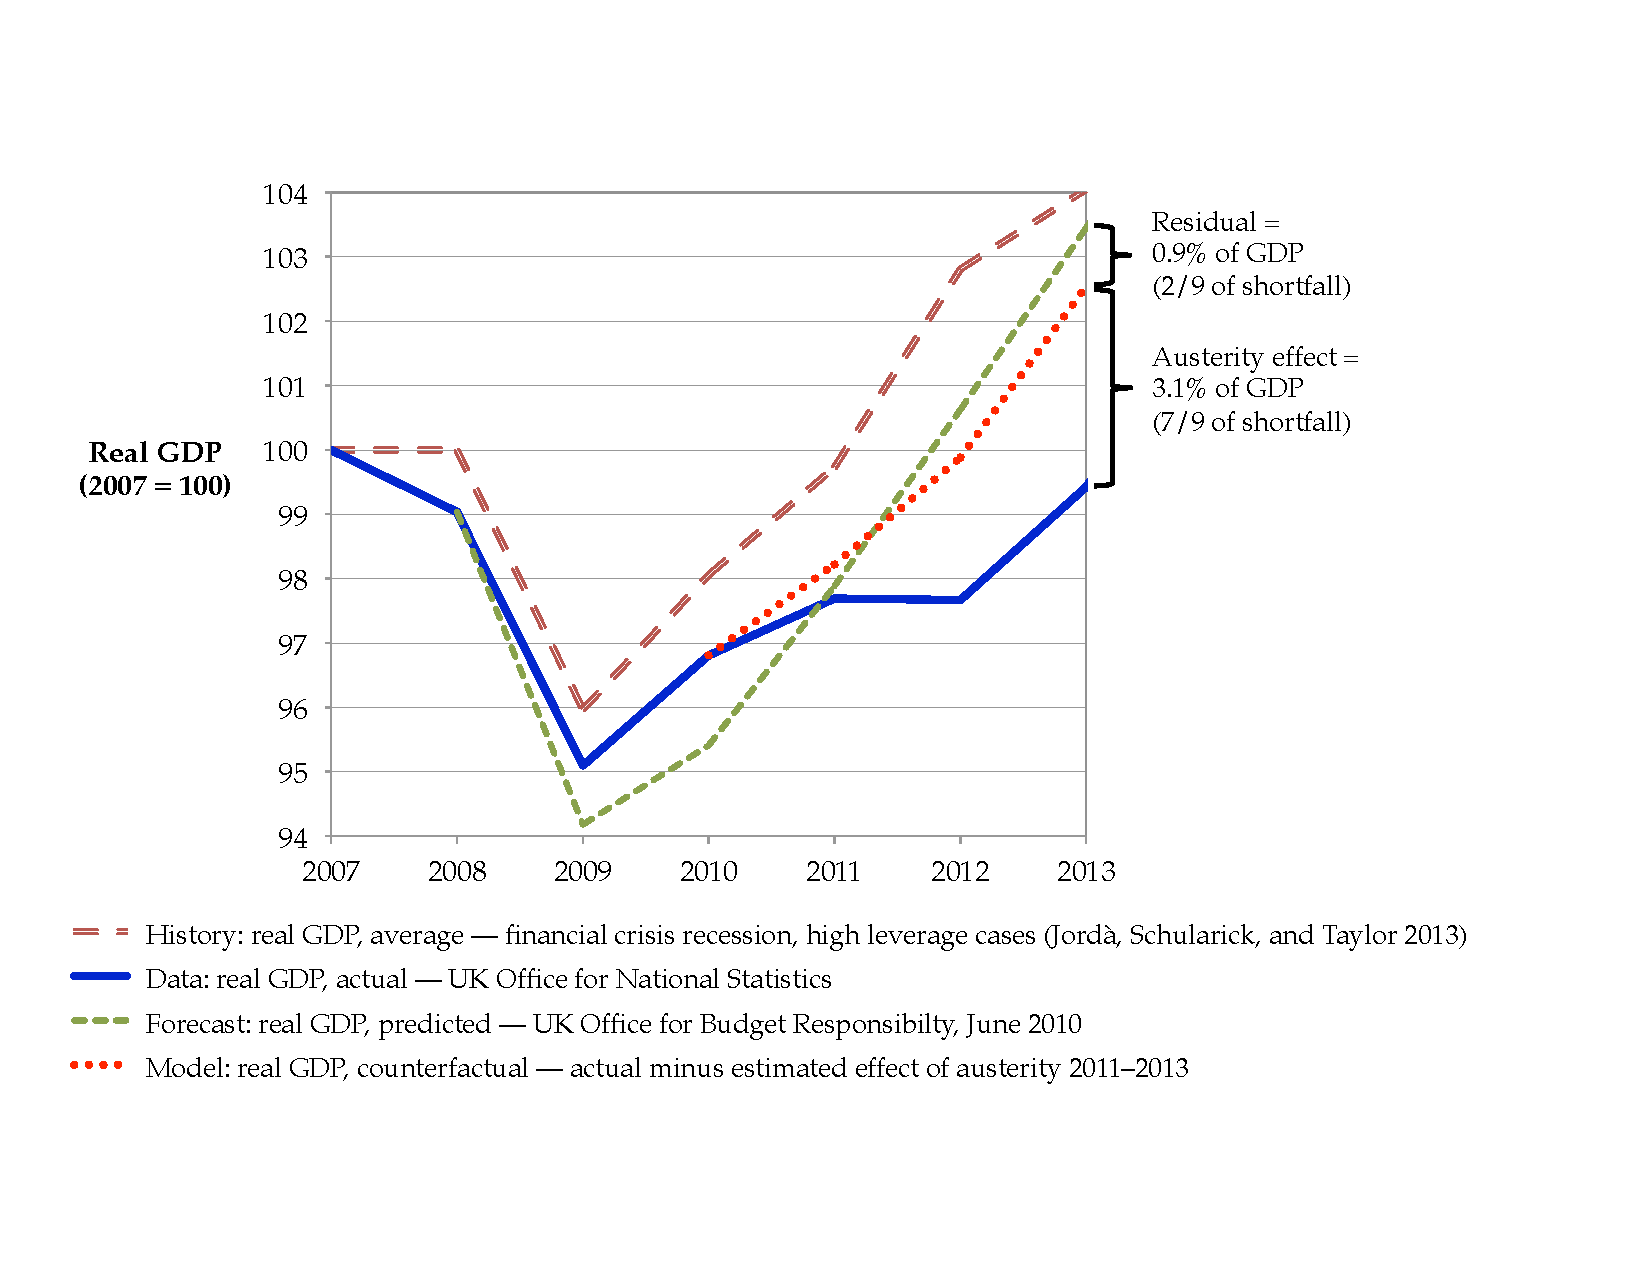
\includegraphics[width=\textwidth]{figure4.pdf}
\end{figure}


\end{document}
